\chapter{Problem 2}
RESULTATER FRA SIMULERING/TESTING

\section{Problem 2a}
	To shorten the length of this report, the code for problem 2 have been put together instead of having seperate code for a, b and c. All plots made in normalized frequency have been from $0-\frac{1}{2}$ since they are real functions. Since the functions are real, the frequency plot is even, and easier to interpret this way.
	
	%\lstinputlisting{Matlab/Oppgave2.m}
	
	The following equation for bitrate was given in the exercise 
	\begin{equation}
		H=\frac{1}{2}log(2\pi e^1\frac{\sigma ^2 _U}{\Delta ^2})
		\label{eq:eq_bit_rate}
	\end{equation}
	
	Solved equation~\ref{eq:eq_bit_rate} for $\Delta ^2$ for use in later equations
	
	\begin{equation}
		\Delta ^2=\frac{2\pi e^1\sigma ^2 _U}{2^{2H}}
	\end{equation}
	
	Equation~\ref{eq:eq_lagrange_mult} is given in the compendium and is used in the process of calculating the optimal filters.
	
	\begin{equation}
		\sqrt{\lambda}=\frac{\int\limits_{-\infty}^{\infty}\sqrt{S_x(f)S_Q(f)}df}{P+\sigma^2_Q}
		\label{eq:eq_lagrange_mult}
	\end{equation}
	
	For the calculation of the lagrange multiplier, the following equation is given in the exercise:
	
	\begin{equation*}
		\sigma^2_Q=\frac{\Delta^2}{12}
	\end{equation*}
	
	The noise is constant over the frequency-band, thus applying
	
	\begin{equation*}
		S_Q(f)=\sigma^2_Q
	\end{equation*}
	
	All inserted in the following equation~\ref{eq:eq_lagrange_mult} that was given in the compendium:

	\begin{equation}
		\sqrt{\lambda}=\frac{\int\limits_{-\frac{1}{2}}^{\frac{1}{2}}\sqrt{\frac{0.19\sigma^2_Q}{1.81-1.8cos(2\pi f)}}df}{1+\sigma^2_Q}
	\end{equation}
	The integral in the equation has to be solved numerically using matlab. The calculated functions and values are used in the following formulas to calculate the optimal transmitter/receiver filters.
	
	\begin{equation}
		|H(f)|^2=\sqrt{\frac{\lambda S_x(f)}{S_Q(f)}}-\lambda
	\end{equation}
	
	\begin{equation}
		|G(f)|^2=\sqrt{\frac{S_N(f)}{\lambda S_x(f)}}-\frac{S_N(f)}{S_x(f)}
	\end{equation}
	
	\lstinputlisting{Matlab/Oppgave2a.m}
	
	\begin{figure}[H]
	  \centering
	  \includegraphics[width=0.75\textwidth]{img/Oppgave2a_freq_G}
	\end{figure}
	
	\begin{figure}[H]
	  \centering
	  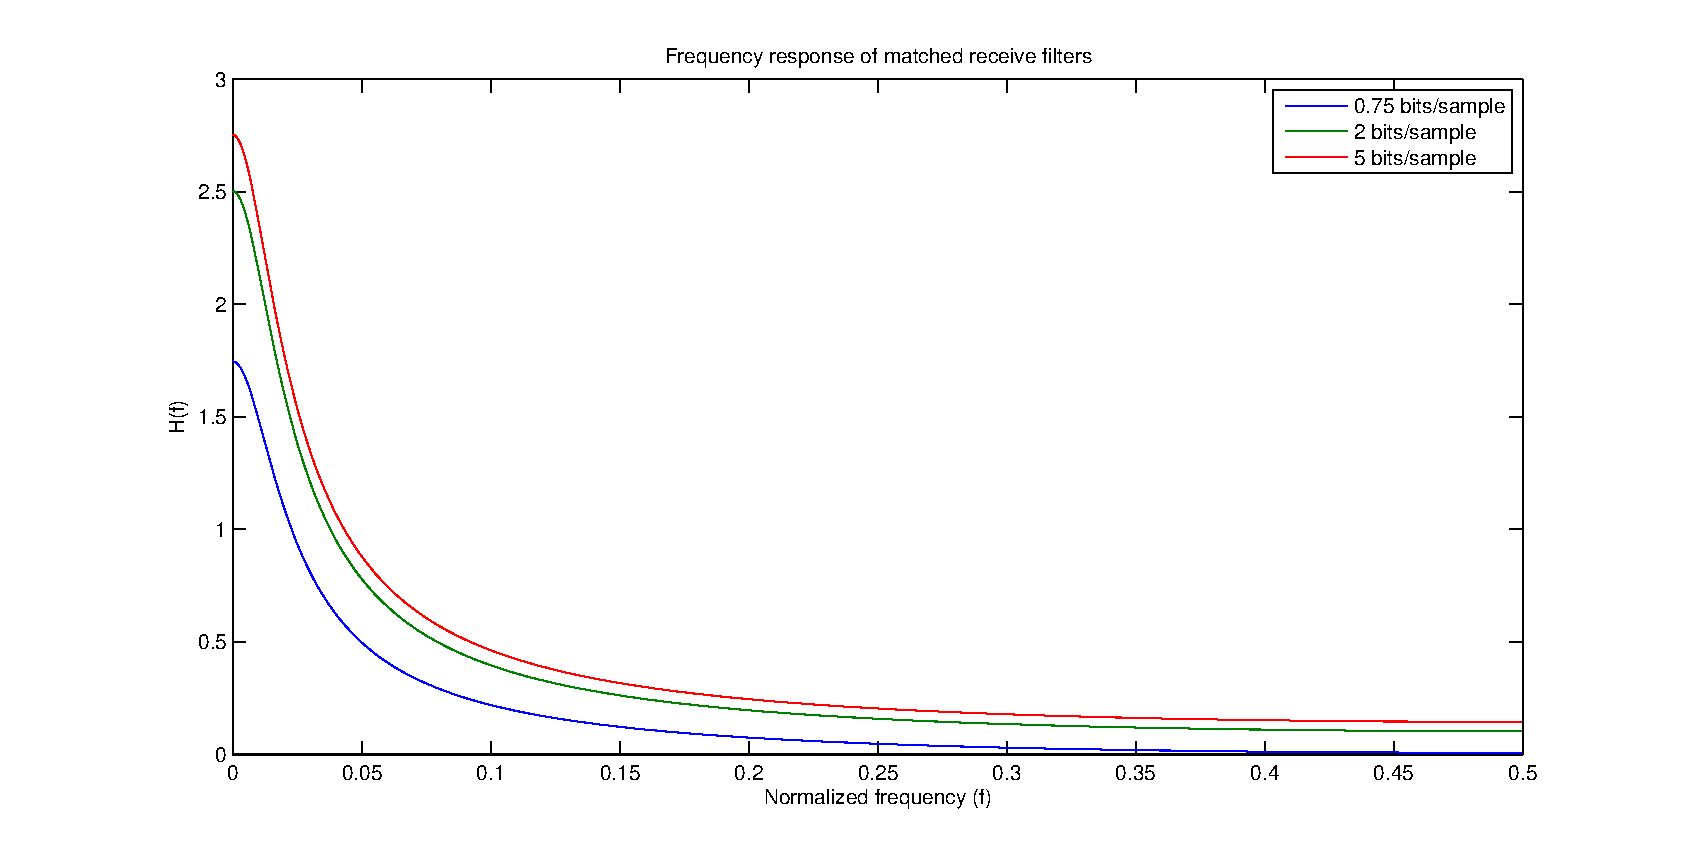
\includegraphics[width=0.75\textwidth]{img/Oppgave2a_freq_H}
	\end{figure}
	
	\begin{figure}[H]
	  \centering
	  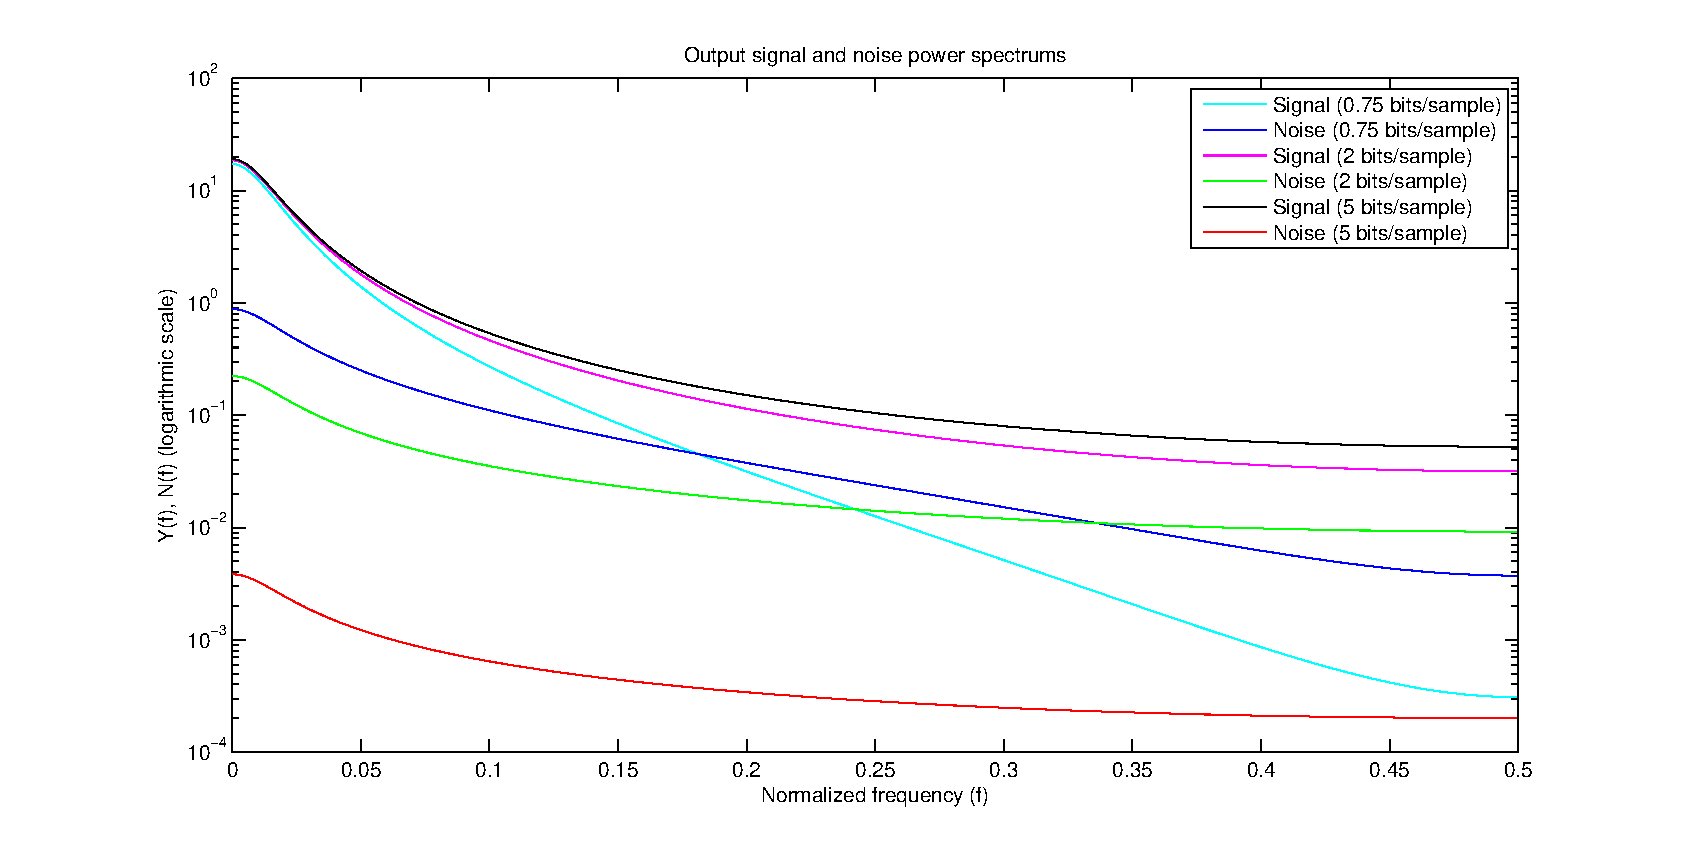
\includegraphics[width=0.75\textwidth]{img/Oppgave2a_sig_noise_freq_out}
	\end{figure}
	
	The SNR for the different values were:
	\begin{table}
		\centering
		\begin{tabular}{l l}
			H & SNR[dB] \\
			0.75 & 9.45 \\
			2 & 14.99 \\
			5 & 32.60 \\
		\end{tabular}
	\end{table}

\section{Problem 2b}

	\lstinputlisting{Matlab/Oppgave2b.m}
	
	\begin{figure}[H]
	  \centering
	  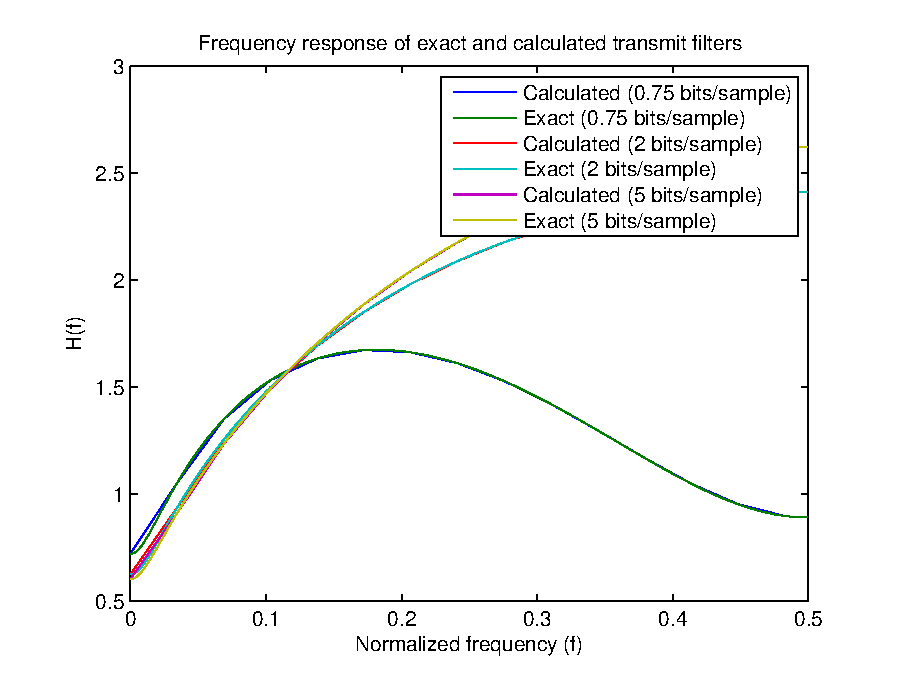
\includegraphics[width=0.75\textwidth]{img/Oppgave2b_freq_G}
	\end{figure}
	
	\begin{figure}[H]
	  \centering
	  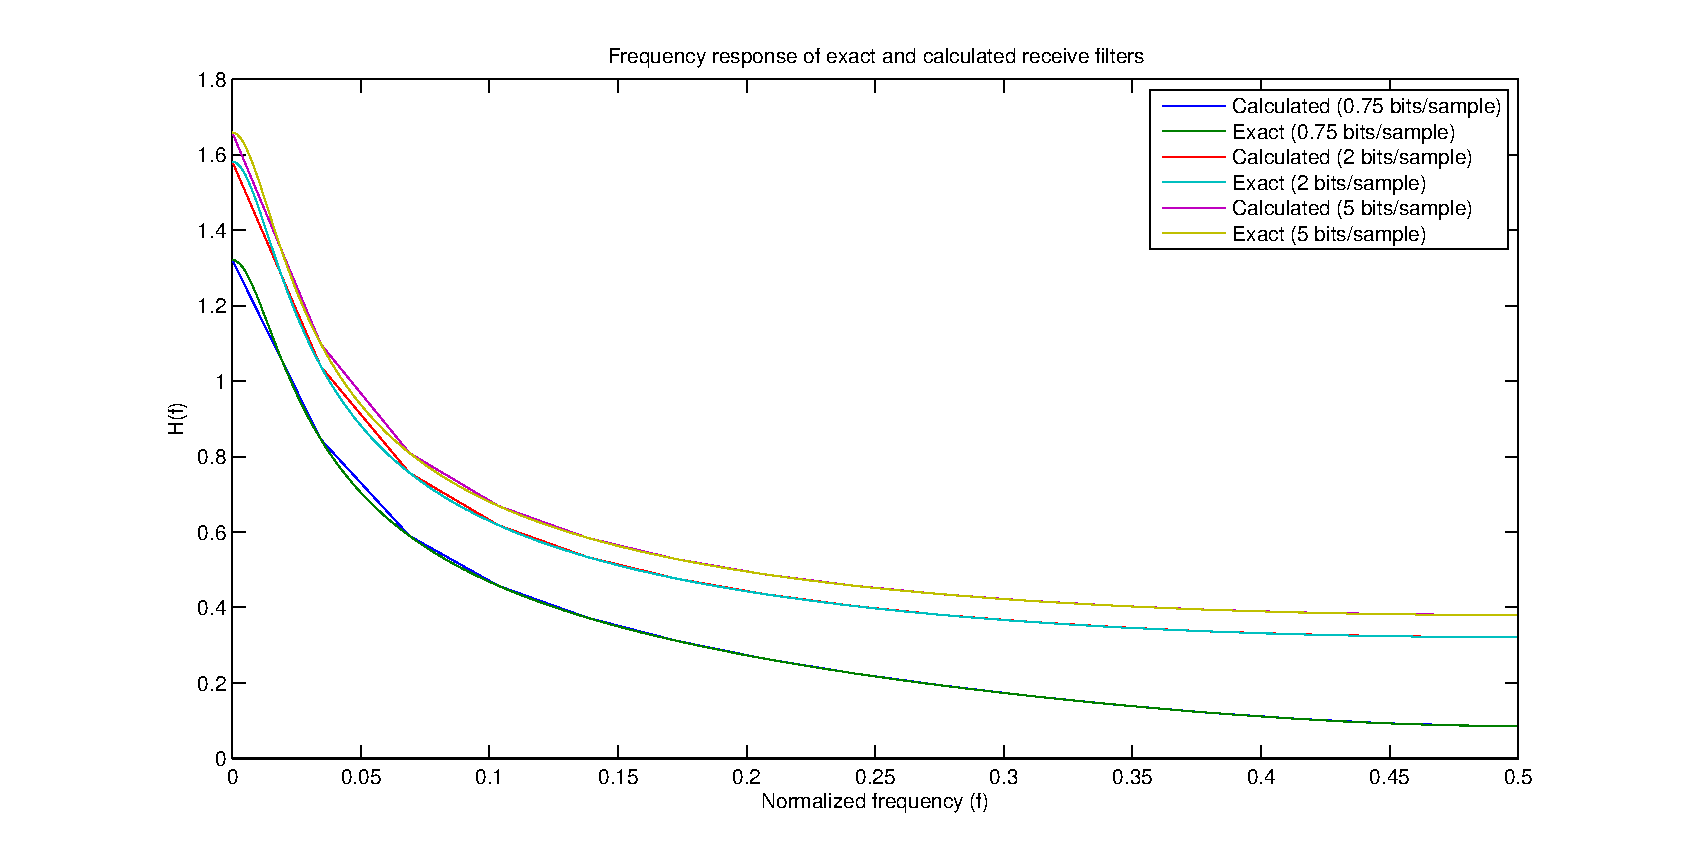
\includegraphics[width=0.75\textwidth]{img/Oppgave2b_freq_H}
	\end{figure}
	
	\begin{figure}[H]
	  \centering
	  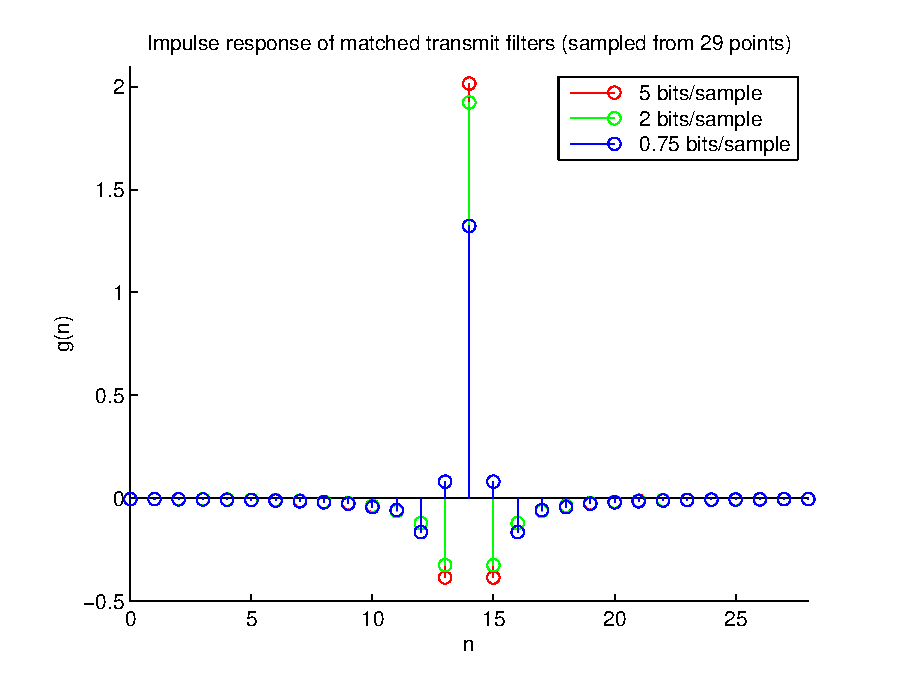
\includegraphics[width=0.75\textwidth]{img/Oppgave2b_impulse_G_diskrete_t}
	\end{figure}
	
	\begin{figure}[H]
	  \centering
	  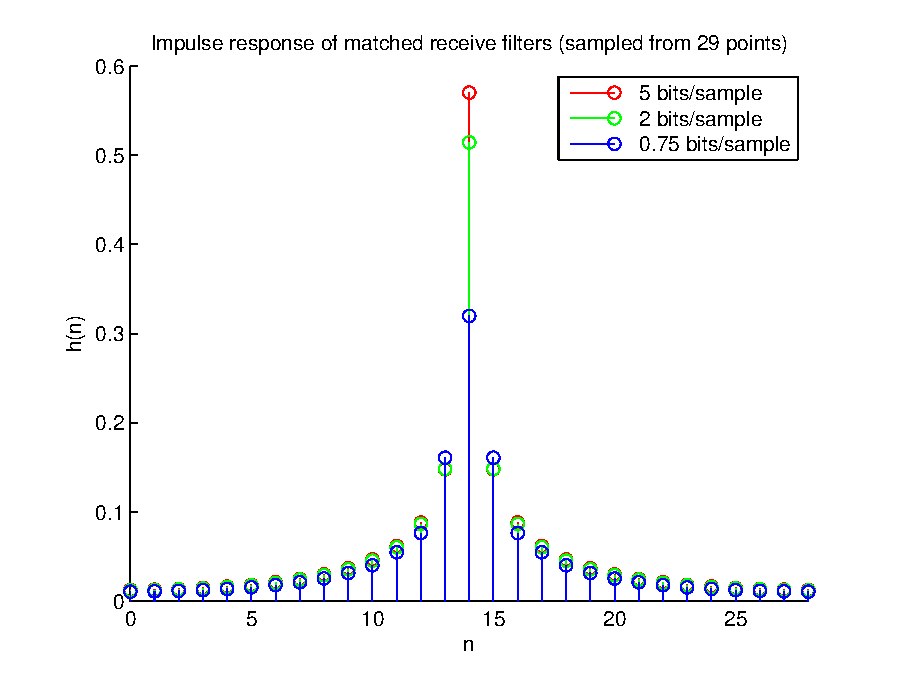
\includegraphics[width=0.75\textwidth]{img/Oppgave2b_impulse_H_diskrete_t}
	\end{figure}
	
	\begin{figure}[H]
	  \centering
	  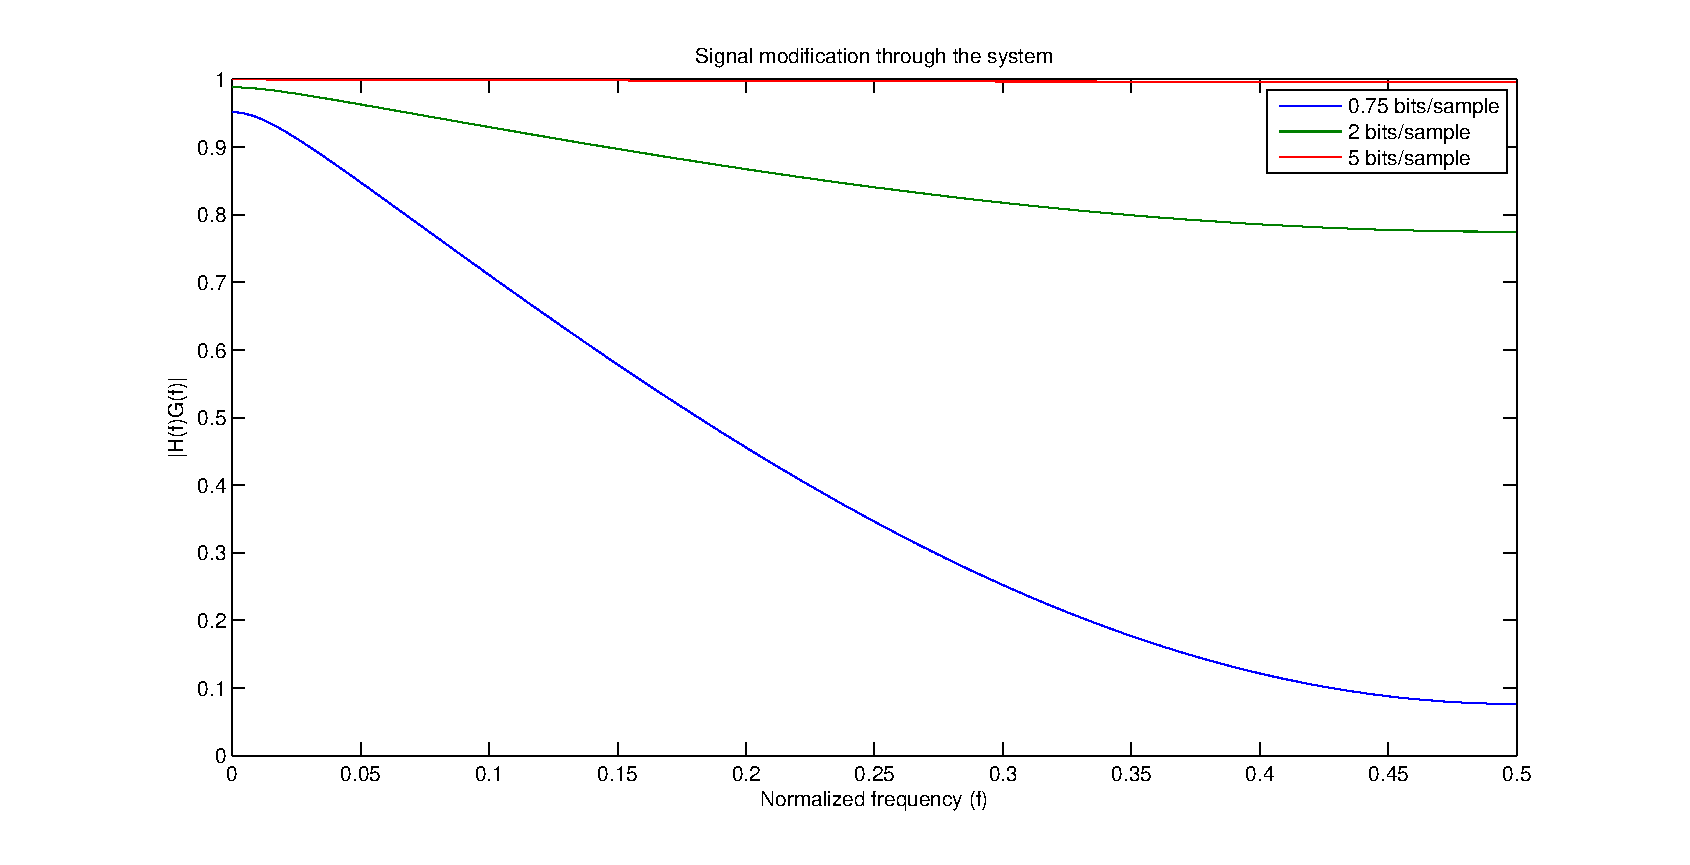
\includegraphics[width=0.75\textwidth]{img/Oppgave2b_signal_mod_x_y}
	\end{figure}

\section{Problem 2c}
